\documentclass[a4paper,10pt]{article}

\usepackage[ansinew]{inputenc}
\usepackage[spanish]{babel}
\usepackage{graphicx}
\usepackage{listings}
\usepackage{appendix}
\usepackage{pdfpages}
\usepackage{array}

\begin{document}

\setcounter{page}{2}

\newpage
\thispagestyle{empty}
\tableofcontents

\newpage
\section{Introducci\'on}

En el presente trabajo pr\'actico se busc\'o familiarizarse con las
herramientas de software que se usar\'an en los siguientes trabajos
pr\'acticos. Estas herramientas son el programa GXemul para simular el
entorno de desarrollo y una m\'aquina MIPS corriendo una versi\'on del
sistema operativo NetBSD. Para ello, se escribieron dos programas en
lenguaje C que permiten convertir archivos de texto desde y hacia
plataformas UNIX. 

\section{Resoluci\'on del problema}
Para la resoluci\'on del ejercicio se realiz\'o una funci\'on llamada
``parser'' encargada de la conversi\'on de archivos de textos desde y hacia 
plataformas UNIX. Para poder lograr la conversi\'on se tuvieron que cambiar los caracteres
\textbackslash n por \textbackslash r\textbackslash n para convertir el formato de archivo de UNIX a DOS y la conversi\'on 
inversa para pasar de DOS a UNIX. 
\newline
Para ejecutar el programa, el comando a utilizar es: ./[nombre de ejecutable] -i [ruta de archivo origen] -o [ruta de archivo destino]
En caso de que no se utilicen las opciones ``i'' (archivo de entrada) y ``o'' (archivo de salida) el programa
utiliza la entrada estandar (stdin) y salida estandar (stdout).

  \subsection{Funcion ``main''}
  En ambos programas se llama a la funci\'on ``parser'' detallada anteriormente, y se retorna el valor de retorno de la misma.
  Lo \'unico que los diferencia es que en ``unix2dos'' el valor de ``finLinea'' toma el valor de \textbackslash n y finLineaNuevo \textbackslash r\textbackslash n, y en ``dos2unix''
  se intercambian esos valores.

  \subsection{Funcion ``parser''}
  Esta funci\'on se encarga de obtener las opciones de ejecuci\'on del programa utilizando la funcion ``getopt'' y, en base
  a eso, llamar a la funci\'on ``traducirFormato'', pasandole los parametros correspondientes.
  \newline
  Para la captura de los par\'ametros opcionales que pueden utilizarse al 
  llamar el programa se decidi\'o utilizar la funci\'on {\bf getopt(int argc,char\*\* argv,char\* options)}. 
  Esta decisi\'on se tomo con el fin de simplificar el c\'odigo necesario para la resoluci\'on del parseo de los
  argumentos; dado que, de este modo, se evita generar c\'odigo que tenga
  en cuenta todas las combinaciones posibles de los mismos. As\'i como
  tambi\'en, para que pueda ser extensible; es decir, pueda expandirse
  f\'acilmente el programa en caso de desear agregar par\'ametros para
  ejecutar el mismo.
  El cuerpo de la funcion 'main' consiste de:
  \begin{itemize}
  \item Se utiliza {\bf getopt} para obtener los par\'ametros con los que se invoca el programa. Y se 
    utilizan flags para determinar en que situaci\'on de las posibles se encuentra.
  \item Se abren los archivos origen, en modo lectura, y destino, en modo escritura escritura (de esta
    forma se crea el archivo, si no existe), en los casos en los que sea necesario. Dado que si la funci\'on
    se invoca en alguna de las posibles combinaciones que permiten stdin y/o stdout, se utiliza dichos 
    archivos.
  \item Se llama a la funcion {\bf traducirFormato}, detallada previamente, con los par\'ametros 
    correspondientes al modo del que fue invocada la aplicaci\'on.
  \item Se cierran ambos archivos, en caso de que corresponda.
  \end{itemize}


  \subsection{Funci\'on ``traducirFormato''}
  Para parsear el archivo de entrada se fue obteniendo caracter a caracter y
  se fue comparando de que no se tratara del fin de linea
  correspondiente a la plataforma del archivo de entrada, de
  encontrarnos en esa situaci\'on se escribe el caracter al archivo de
  salida. Si nos encontramos en el caso de fin de linea se escribe en el
  archivo de salida el fin de linea de la otra plataforma. 
  El encabezado de la funci\'on es el siguiente:
  \newline
  {\bf void parser(FILE * origen, FILE * destino, char *finLinea, char *finLineaNuevo)}
  \newline
  Los par\'ametros que recibe son:

  \begin{itemize}
  \item {\bf FILE *origen:}
    Descriptor del archivo origen. Debe existir y estar abierto correctamente.
  \item {\bf FILE *destino:}
    Descriptor del archivo destino, en el que se almacenara el archivo resultante. Debe estar abierto correctamente.
  \item {\bf char *finLinea:}
    Cadena que almacena la cadena de fin de linea del archivo origen.
  \item {\bf char *finLineaNuevo:}
    Cadena que almacena la cadena de fin de linea del archivo destino.
  \end{itemize}

\section{Compilaci\'on en NetBSD}
  Para poder compilar desde NetBSD y obtener el c\'odigo MIPS generado por el compilador, se debe ejecutar:
  \newline
  {\bf guestOS\# gcc -Wall -O0 -S -mrnames unix2dos.c} 
  \newline
  {\bf guestOS\# gcc -Wall -O0 -S -mrnames dos2unix.c}
  \newline
  Donde:
  \begin{itemize}
  \item {\bf-S:} detiene al compilador luego de generar el assembly.
  \item {\bf-mrnames} (solo para MIPS): indica al compilador que genere la salida utilizando nombre de 
    registro en lugar de n\'umero de registro.
  \item {\bf-O0:} No aplica optimizaciones.
  \end{itemize}
  A continuaci\'on el c\'odigo assembly:
  \subsection{unix2dos}
    \lstset{numbers=left, frame=single, breaklines=true}
    \lstinputlisting{../Codigo/dos2unix.s}
  \subsection{dos2unix}
    \lstset{numbers=left, frame=single, breaklines=true}
    \lstinputlisting{../Codigo/unix2dos.s}

\section{Casos de prueba}

En la siguiente secci\'on se detallaran los distintos archivos utilizados para probar el funcionamiento del
programa. Para ello se adjuntaran imagenes de corridas de los mismos; en donde se ense\~{n}a el dump del 
archivo origen, en formato ASCII con barra invertidas para los caracteres de escape, y luego el del 
archivo destino.

  \subsection{Distintas formas de invocaci\'on}
    \subsubsection{Prueba 1}
    Invocaci\'on del programa con par\'ametros -i y -o definidos:
    \begin{itemize}
      \item \textbf{dos2unix}
      \item \textbf{unix2dos}
    \end{itemize}

    \subsubsection{Prueba 2}
    Invocaci\'on del programa con par\'ametros -i definido:
    \begin{itemize}
      \item \textbf{dos2unix}
      \item \textbf{unix2dos}
    \end{itemize}
  
    \subsubsection{Prueba 3}
    Invocaci\'on del programa con par\'ametros -i igual a ``-'' (flujo est\'andar stdin):
      \begin{itemize}
      \item \textbf{dos2unix}
      \item \textbf{unix2dos}
      \end{itemize}

    \subsubsection{Prueba 4}
    Invocaci\'on del programa con par\'ametros -i definido y -o igual a ``-'' (flujo est\'andar stdout):
      \begin{itemize}
      \item \textbf{dos2unix}
      \item \textbf{unix2dos}
      \end{itemize}

    \subsubsection{Prueba 5}
    Invocaci\'on del programa con par\'ametros -i y -o indefinido (flujo est\'andares implicitos):
      \begin{itemize}
      \item \textbf{dos2unix}
      \item \textbf{unix2dos}
      \end{itemize}

    \subsubsection{Prueba 6}
    Invocaci\'on del programa con entrada por stdin y salida por stdout:
      \begin{itemize}
      \item \textbf{dos2unix}
      \item \textbf{unix2dos}
      \end{itemize}

  \subsection{Distintos archivos de prueba}
    \subsubsection{Prueba 1}
    Utilizaci\'on de un archivo de origen vac\'io:
      \begin{itemize}
      \item \textbf{dos2unix}
      \item \textbf{unix2dos}
      \end{itemize}

    \subsubsection{Prueba 2}
    Utilizaci\'on de un archivo de un archivo simple:
      \begin{itemize}
      \item \textbf{dos2unix}
      \item \textbf{unix2dos}
      \end{itemize}

    \subsubsection{Prueba 3}
    Utilizaci\'on de un archivo de un archivo complejo:
      \begin{itemize}
      \item \textbf{dos2unix}
      \item \textbf{unix2dos}
      \end{itemize}

    \subsubsection{Prueba 4}
    Conversi\'on de un archivo de un formato al otro, y el resultado convertirlo al formato original.
      \begin{itemize}
      \item \textbf{dos2unix}
      \item \textbf{unix2dos}
      \end{itemize}
\section{Conclusiones}
Completar...


%APENDICES
\appendix
\newpage
\section{C\'odigo Fuente}
  \subsection{unix2dos.c}
    \lstset{numbers=left, frame=single, breaklines=true}
    \lstinputlisting{../Codigo/unix2dos.c}
  \subsection{dos2unix.c}
    \lstset{numbers=left, frame=single, breaklines=true}
    \lstinputlisting{../Codigo/dos2unix.c}
  \subsection{conversor.c}
    \lstset{numbers=left, frame=single, breaklines=true}
    \lstinputlisting{../Codigo/conversor.c}

\newpage
\section{Enunciado}
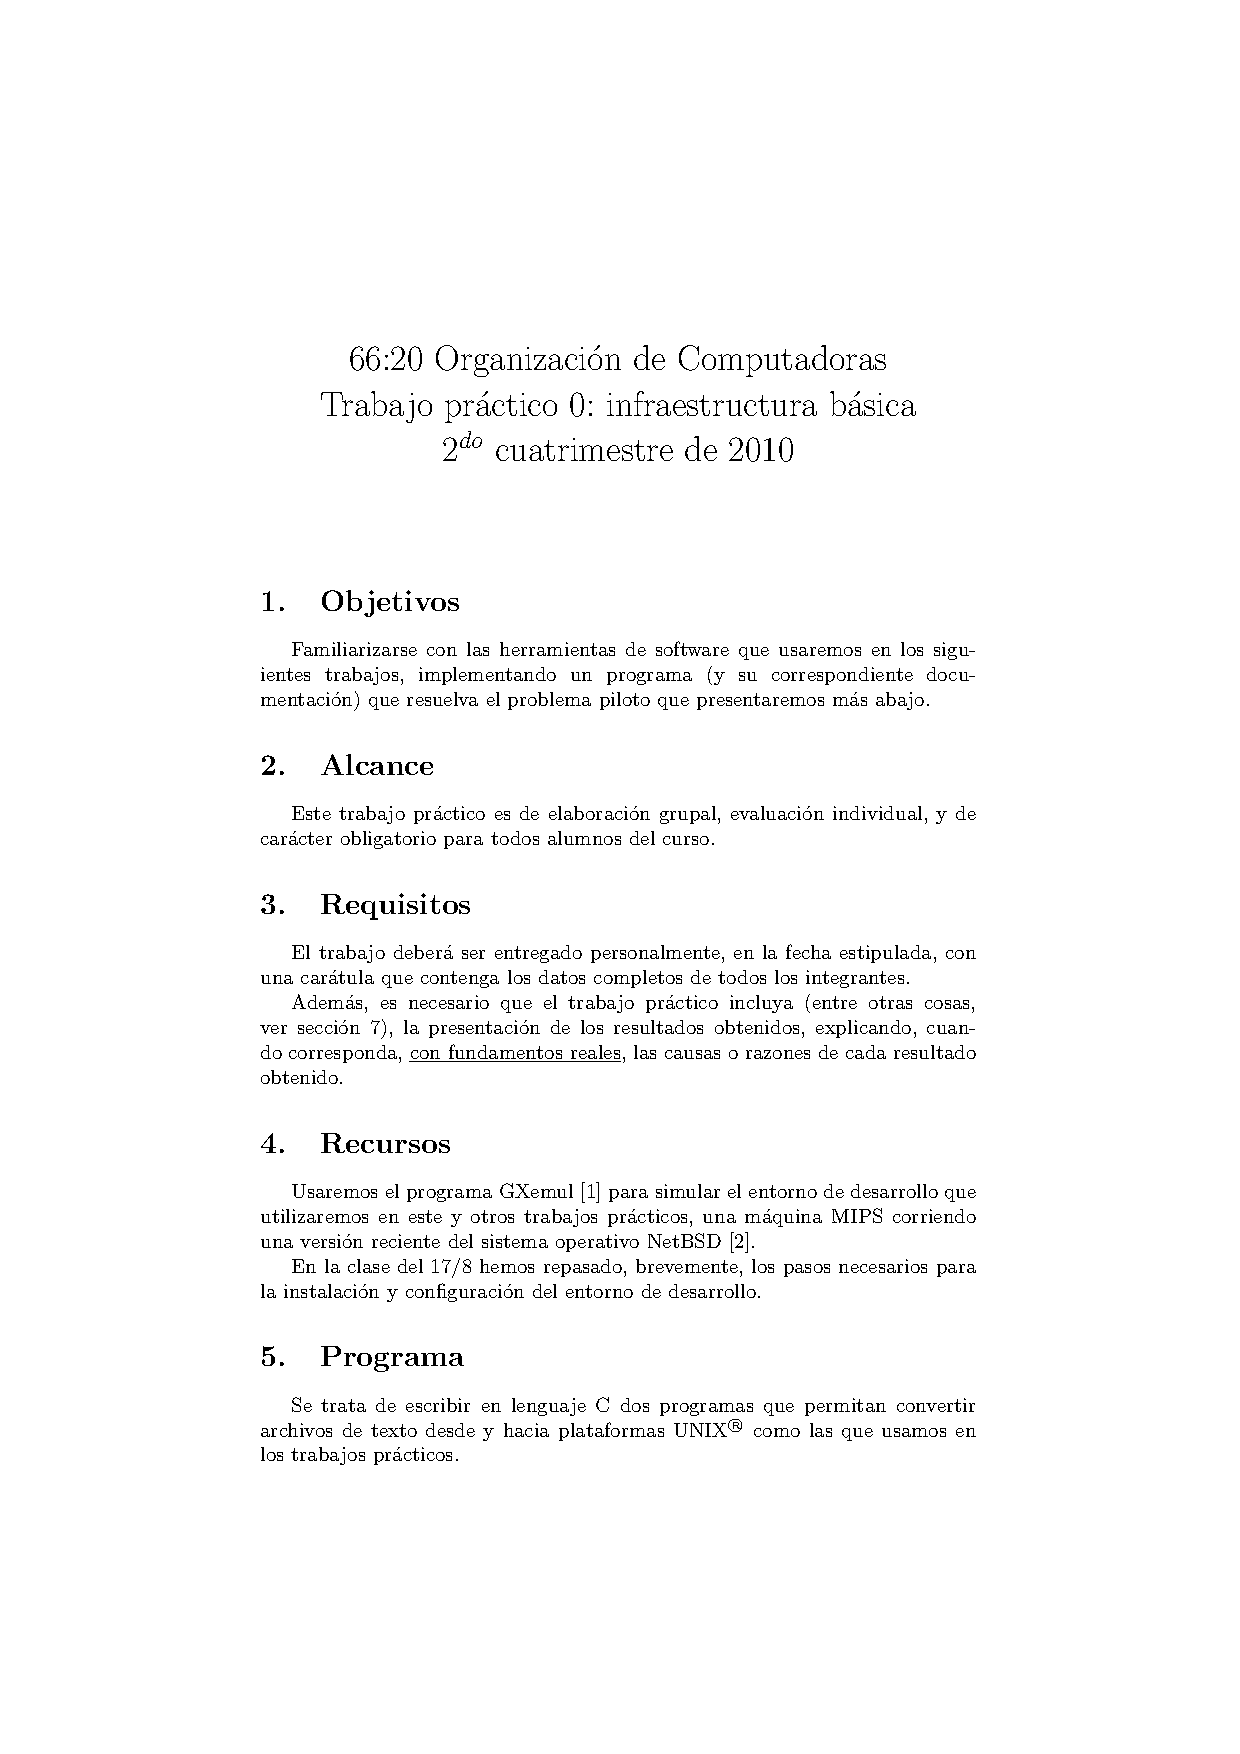
\includepdf[pages=1-3, scale=0.9, pagecommand={\thispagestyle{plain}}]{../tp0-2010-2q.pdf}

\end{document}
